\section{Future Work}\label{sec:conclusion:future_work}
First, we will introduce several overarching recommendations for the field moving into a future where soft robots are an essential contributor to our daily lives.
Next, we outline several concrete avenues for future research building directly on this thesis.

\subsection{General Recommendations}
% \begin{itemize}
%     \item Various commercial platforms to unlock more (high-level) algorithmic research
%     \item Demonstrate practical uses-cases in the field (and not just on the breadboard/lab) where soft robots are performing better than rigid manipulators / Cobots along some dimension
%     \item User studies that soft robots are more safe, and are (hopefully) are also perceived~\citep{jorgensen2022soft} to be more natural, safer and friendly.
% \end{itemize}

% Historically, the primary focus of soft robotic research has been on their design and actuation. Even though there has been increased attention on the modeling and control of soft robots in recent years (since \~2017), we find that the computational intelligence of soft robots is still underinvestigated. Specifically, there is little to no research on important topics such as perception, high-level motion planning, task assignment, reasoning, etc., with algorithms that are tailored to soft robotic scenarios, such as operation in human-centric environments or appreciating contact with the environment.
Historically, soft robotics research has primarily focused on design and actuation. Although the modeling and control of soft robots have garnered more attention in recent years, we find that cognitive intelligence for soft robots remains still underexplored. In particular, there is a notable lack of research on critical areas such as perception, high-level motion planning, task assignment, and reasoning—with tailored algorithms suited for soft robotic applications in human-centric environments or scenarios involving physical contact.

% In our opinion, one of the reasons for the missing of such high-level computational intelligence research is the lack of commercially accessible continuum soft robots, compared to the commercially available rigid manipulators, \glspl{Cobot}, and quadrupeds as examples. Therefore, it is largely infeasible for a lab that has its core expertise in areas relating to computational intelligence to begin soft robotic research as it would take many years to acquire the necessary knowledge to build a competitive and robust soft robot prototype.
% We hypothesize that widespread access to (affordable) continuum soft robots will lead to an exponential increase in the computational intelligence of soft robots within just a few years.
We believe one reason for this gap in high-level cognitive intelligence research is the scarcity of commercially available continuum soft robots compared to rigid manipulators, \glspl{Cobot}, and quadrupeds. This limitation makes it challenging for labs specializing in cognitive intelligence to venture into soft robotics, as developing a competitive, robust prototype requires years of expertise. We hypothesize that broader access to affordable continuum soft robots would catalyze rapid, exponential progress in the cognitive/computational intelligence of soft robots.

% The availability of such more reliable, robust and longer-living commercial soft robots should also allow for the conduct of extensive field trials as so far, the experimental validation of soft robots has been constrained to breadboard/lab tests.
% Specifically, we should aim as fast as possible to demonstrate that soft robots are quantitatively more performant/beneficial along at least one dimension in an extensive field trial compared to standard rigid manipulators/\glspl{Cobot}.
% In our opinion, this is essential for keeping and increasing the investment into soft robot research and achieving a thriving field~\citep{hawkes2021hard} and development and preventing us from facing an "\emph{robotic winter}," as it has been the case for \gls{AI} in the past~\citep{muthukrishnan2020brief}.
Furthermore, the emergence of more reliable, robust, and longer-lasting commercial soft robots would enable extensive field trials, moving beyond the breadboard and lab environments that have thus far dominated experimental validation. Demonstrating that soft robots outperform standard rigid manipulators or \glspl{Cobot} in at least one measurable dimension is crucial. Such evidence is essential for sustaining and increasing investment in soft robotics research, fostering a vibrant field, and avoiding a potential “robotic winter” reminiscent of past challenges in \gls{AI}~\citep{muthukrishnan2020brief}.

% Along with these field trials, we would like to see user studies that demonstrate clearly that soft robots are safer than \glspl{Cobots} along with setting clear requirements for \emph{safe} soft robots, possibly conditioned on various applications.
% Similarly, we identify the need for more studies that investigate if soft robots are \emph{perceived} safer and more friendly than traditional rigid robots (compare to the subfield of \emph{social robotics}~\citep{breazeal2016social}). Initial results found that soft robots are not perceived to be more natural than rigid robots, but additional studies in various settings and comparing different soft robot designs are required.
In addition to field trials, we advocate for user studies that clearly establish soft robots as safer than \glspl{Cobot}, along with defining explicit safety requirements—potentially tailored to various relevant applications, such as assisting the elderly with \glspl{ADL} or collaborative manufacturing. More research is also needed to determine whether soft robots are perceived as safer and friendlier than traditional rigid robots.
% , a topic that aligns with the objectives of social robotics. 
% Essentially, we required an increased investigation into \emph{social soft robots}, as it is already done for their rigid counterparts~\citep{breazeal2016social}.
Essentially, further investigation into \emph{social soft robots} is needed—mirroring the research already conducted on their rigid counterparts~\citep{breazeal2016social}.
Although initial findings suggest that soft robots may not be inherently perceived as more natural than rigid ones~\citep{jorgensen2022soft}, further investigations across diverse settings and designs are warranted~\citep{pasquier2025study}.

% In the following, we will outline several specific directions for future work that directly connect to the research presented in this thesis.
% They all center around increasing the \emph{physical-intelligence}, including improving the precision, dexterity, and ability to tackle complex real-world tasks that consist of a long sequence of precise and dynamic motions with a specific focus on human-centric environments while ensuring that safety is guaranteed.
% Ultimately, the practical usefulness of soft robots need to be increase by several order of magnitudes in order to be an economically viable option and this is what the research community should focus on in the next years.
In the following section, we outline several future research directions directly linked to the work presented in this thesis. These avenues focus on enhancing the physical intelligence of soft robots by improving their precision, dexterity, and capability to handle complex, sequential real-world tasks—especially in human-centric environments where safety is paramount. Ultimately, increasing the practical utility of soft robots by several orders of magnitude is necessary for soft robots to become an economically viable option, and this challenge should be a primary focus for the research community in the coming years.

% Despite significant progress, several key challenges remain for safe and effective soft robot control: (1) controllers must explicitly address safety risks, (2) high-level motion policies must ensure stable and compliant behavior, and (3) computationally tractable methods are needed for co-designing the robot’s body and brain. These challenges are discussed in detail below.


% \subsection{Safety Metric}
\subsection{Towards a Universally Accepted Safety Metric}
% For future work, we advise an experimental validation of the safety metric proposed in Chapter~\ref{chp:safetymetric}. This should involve a large-scale experimental characterization of the collision characteristics of soft robots, including various designs (e.g., silicon and helicoid soft robots) and different actuation methods (e.g., pneumatic, tendon-driven), and verification if the maximum contact force/pressure predicted by the safety metric matches the experimental measurements.
% Furthermore, controlled user studies should investigate suitable thresholds on the maximum force/pressure for various body areas, such as was done for collaborative robots~\citep{muttray2014kollaborierende}.
% This future research could enable the development of an internationally recognized standard (e.g., ISO) that soft robots need to be certified as being sufficiently safe for a set of applications.
% Furthermore, we encourage an investigation of how the proposed safety metric could be used to achieve safety-aware control. Possibly approaches could, for example, leverage \gls{MPC}, \glspl{CBF}~\cite{ames2016control}, or the derivation of conditions for safe operation (e.g., maximum velocity, torque, stiffness, reflected mass, etc.) via a safety map~\cite{mansfeld2018safety}.
For future work, we recommend experimentally validating the safety metric introduced in Chapter~\ref{chp:safetymetric}. This validation should involve a comprehensive experimental characterization of the collision properties of soft robots, covering various designs (e.g., silicon and helicoid soft robots) and different actuation methods (e.g., pneumatic, tendon-driven), and should verify whether the maximum contact force/pressure predicted by the metric corresponds with experimental measurements. Additionally, controlled user studies should determine appropriate thresholds for maximum force/pressure across different body areas, similar to the approach taken for collaborative robots~\citep{muttray2014kollaborierende}. Such research could pave the way for establishing an internationally recognized standard (e.g., ISO) that certifies soft robots as sufficiently safe for specific applications. Moreover, we encourage exploring how the proposed safety metric can be integrated into safety-aware control strategies~\citep{wong2025contact}. Potential approaches might include leveraging \gls{MPC}, \glspl{CBF}~\citep{ames2016control, wong2025contact}, or developing conditions for safe operation (e.g., maximum velocity, torque, stiffness, reflected mass, etc.) through a safety map~\citep{mansfeld2018safety}.

% \subsection{Modeling and Control of HSA Robots}
\subsection{Towards Dexterous and Precise HSA Robots}
% In Chapter~\ref{chp:hsacontrol}, we proposed several control approaches for planar \gls{HSA} and experimentally verified their efficacy.
% However, the presented control framework exhibits limitations along several axes: (a) it is designed for motions in a plane, (b) it is restricted to one-segment \gls{HSA} robots, (c) it is tailored towards setpoint regulation but not trajectory tracking, (d) it does not explicitly account for the hysteresis that HSA robots exhibit~\citep{truby2021recipe} and requires a \emph{calibration} of the rest strain before each control experiment.
% Specifically, we would like to in the future exploit the twisting motion primitives, as shown in Fig.~\ref{fig:hsamodel:motion_primitives}, which makes \gls{HSA} robots rather unique in the domain of soft robotics.
In Chapter~\ref{chp:hsacontrol}, we introduced several control strategies for planar \gls{HSA} robots and demonstrated their effectiveness experimentally. Nonetheless, this control framework has several limitations: (a) it is confined to planar motions, (b) it applies only to single-segment \gls{HSA} robots, (c) it is geared toward setpoint regulation rather than trajectory tracking, and (d) it does not explicitly account for the hysteresis inherent to HSA robots~\citep{truby2021recipe}, necessitating a calibration of the rest strain before each experiment. In particular, future work should explore the twisting motion primitives illustrated in Fig.~\ref{fig:hsamodel:motion_primitives}, which contribute to the unique behavior of \gls{HSA} robots within soft robotics.

% To tackle (a), a kinematic parametrization describing the 3D motion of \gls{HSA} robot is required. Here, future work could build on the \gls{SPCS} model proposed in Chapter~\ref{chp:hsamodel} for describing the deformation of each \gls{HSA} rod and subsequently derive the closed-chain dynamics by enforcing Pfaffian constraints~\citep{armanini2021discrete} to prevent any drifting of the redundant \glspl{DOF} of the kinematic model.
% Concerning (b), very recent work by \citet{good2025torque} demonstrated how multi-segment \gls{HSA} robots could be achieved by actuating the distal segments through servo motors attached at the robot base via Bendable Extendable Torque Resistant (BETR) shafts which reduce the inertia that is in motion, compared to a \emph{naive} solution of attaching the motors at the proximal end of each segment. 
% While extending the model and controllers to the multi-segment case should be straightforward and has been shown in literature for standard continuum soft robots~\cite{della2020model}, new actuation models are likely necessary to capture the peculiar characteristics of the BETR shafts.
% With respect to (c), the main challenge of devising trajectory tracking controllers is the underactuated nature of the robot model: Trajectory tracking controller for the fully actuated case are already established in literature~\citep{della2020model}. Recent work by \citet{soleti2025model} presents the trajectory tracking control of an underactuated soft robot based on dielectric elastomers. It should be possible to transfer this control approach to \gls{HSA} robots.
% Finally (d), the hysteretic behavior of \gls{HSA} robots could be captured by the Bouc-Wen~\citep{bouc1967forced, wen1976method} or similar models.
% Then, a nonlinear observer~\citep{shao2023model} could be derived for estimating online the (hidden) hysteretic displacement based on the recent state evaluation.
% Finally, an optimal control approach, such as \gls{MPC}, could take into account the hysteretic state of the system when devising the next control action.

To address limitation (a), a kinematic parameterization that captures the three-dimensional motion of \gls{HSA} robots is needed. Future research could build on the \gls{SPCS} model introduced in Chapter~\ref{chp:hsamodel}—which describes the deformation of each HSA rod—by deriving closed-chain dynamics through the enforcement of Pfaffian constraints~\citep{armanini2021discrete, tsounis2025solving} to eliminate drift in the redundant degrees of freedom.

Regarding limitation (b), recent work by \citet{good2025torque} has shown that multi-segment \gls{HSA} robots can be realized by actuating the distal segments with servo motors mounted at the robot base via Bendable Extendable Torque Resistant (BETR) shafts. This design reduces the inertia in motion compared to the more naive approach of placing motors at the proximal end of each segment. While extending existing models and controllers to accommodate multi-segment systems appears straightforward—as evidenced by work on standard continuum soft robots~\citep{della2020model}—new actuation models will likely be necessary to capture the unique properties of BETR shafts accurately.

Concerning limitation (c), the main challenge in developing trajectory-tracking controllers lies in the underactuated nature of the robot model. Although trajectory tracking controllers for fully actuated systems are well-established in the literature~\citep{della2020model}, recent research by \citet{soleti2025model} on trajectory tracking for underactuated soft robots based on dielectric elastomers suggests that similar strategies could be adapted for \gls{HSA} robots.

\begin{figure}[ht]
    \centering
    \subfigure[\gls{HSA} rod characterization by \citet{truby2021recipe}]{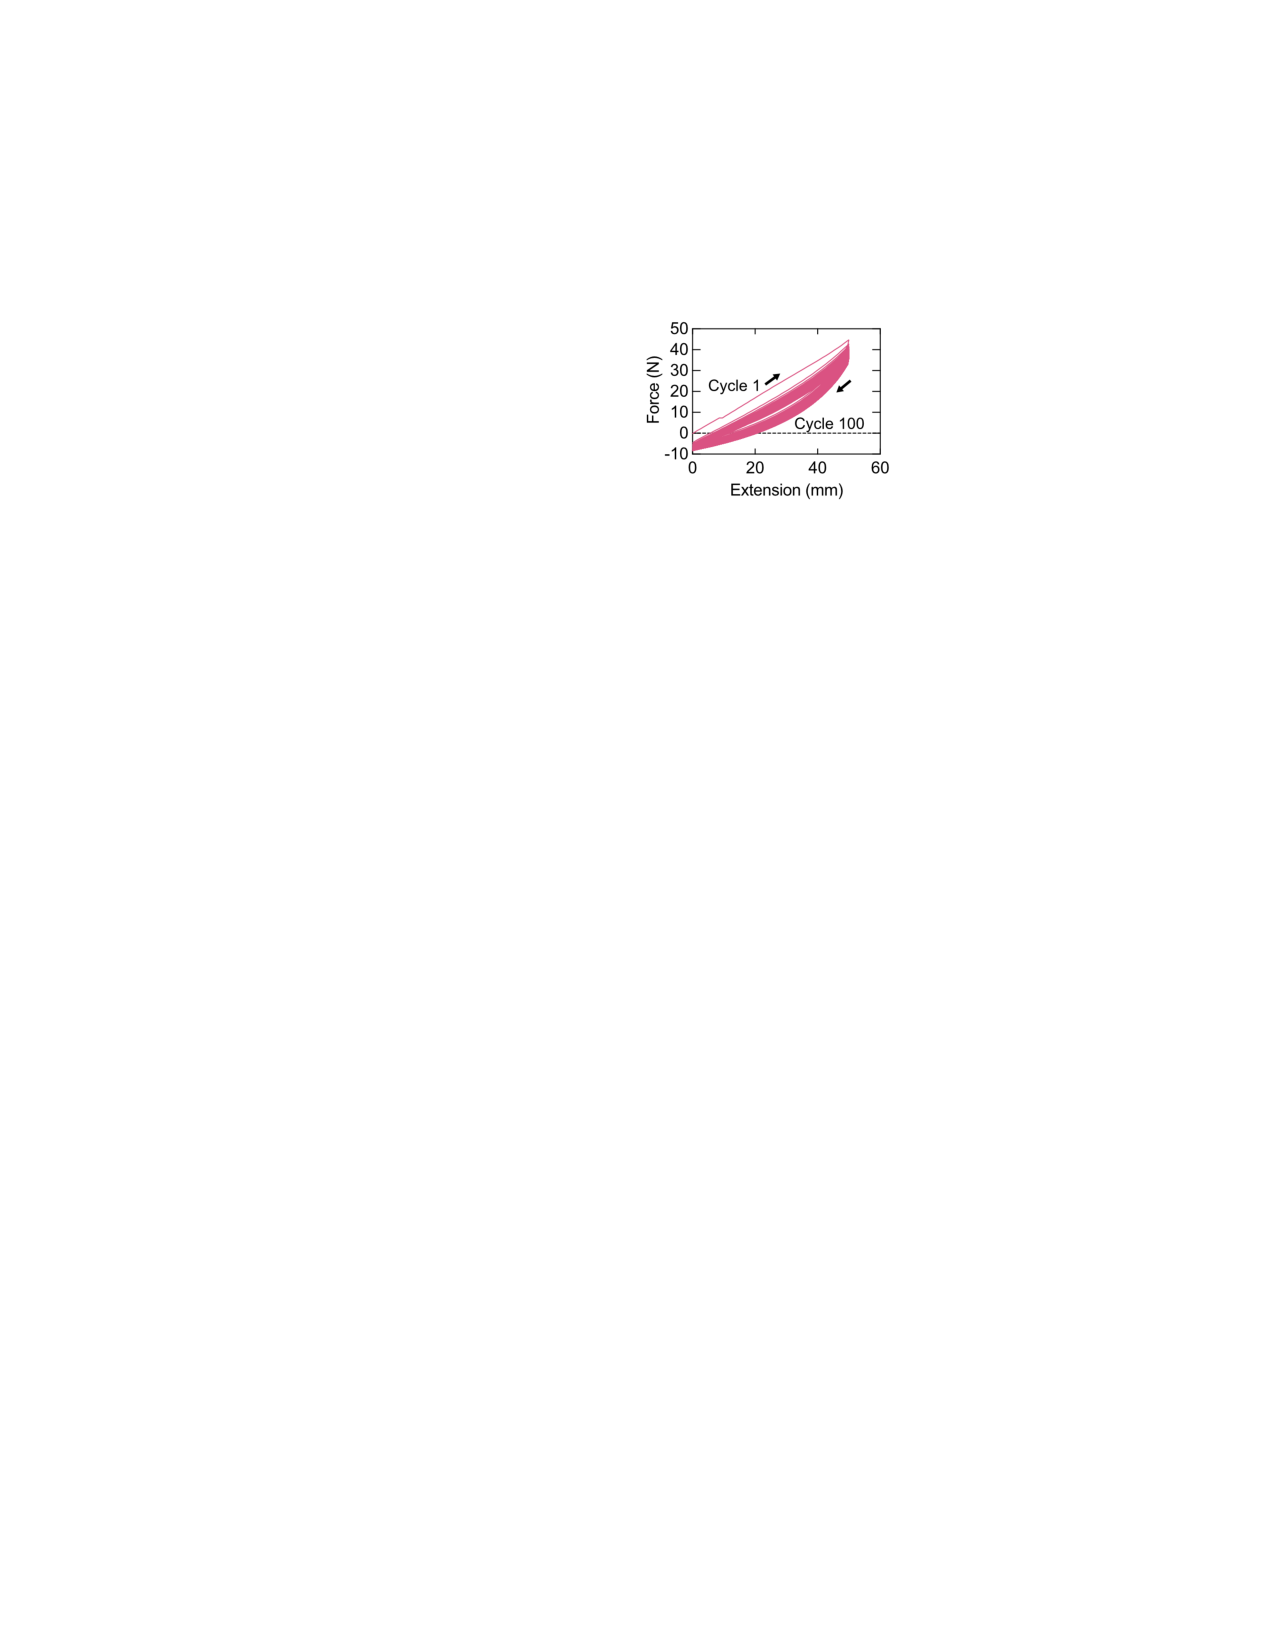
\includegraphics[width=0.44\linewidth]{conclusion/figures/future_work/hsa_control/hsa_extension_test_truby.pdf}}
    \subfigure[\gls{HSA} rod behavior simulated with a Bouc-Wen model]{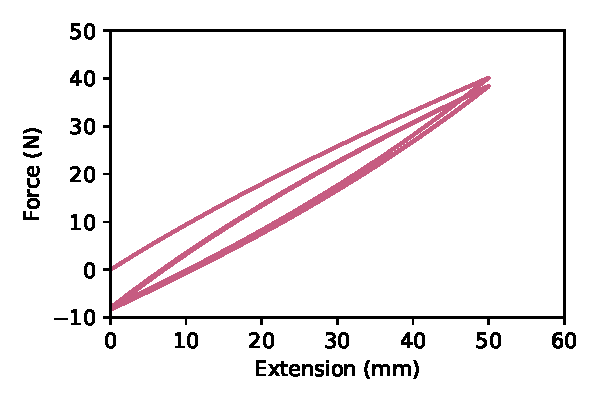
\includegraphics[width=0.48\linewidth, trim={5, 5, 5, 5}]{conclusion/figures/future_work/hsa_control/hsa_tensile_extension_test_force_displacement_curve.pdf}}
    \caption{\textbf{Left:} Mechanical characterization of FPU \gls{HSA} rods by \citet{truby2021recipe}. \textbf{Right:} Preliminary simulation of a \gls{HSA} rod based on the model derived in Chapter~\ref{chp:hsamodel} augmented with a Bouc-Wen model to capture hysteretic behavior.}
    \label{fig:conclusion_future_work:hsa_control:hysteresis}
\end{figure}

Finally, to overcome limitation (d), the hysteretic behavior of \gls{HSA} robots could be modeled using the Bouc-Wen framework~\citep{bouc1967forced, wen1976method} or related approaches. As shown in Fig.~\ref{fig:conclusion_future_work:hsa_control:hysteresis}, preliminary results show that a Bouc-Wen model with $\alpha=0.1$, $\beta=0.25$, and $\gamma=-0.75$ representing strain hardening can capture the hysteretic behavior of \gls{HSA} rods, as experimentally characterized by \citet{truby2021recipe} relatively well.
A nonlinear observer~\citep{shao2023model} could then be developed to estimate the hidden hysteretic displacement in real-time based on the current state. Ultimately, incorporating an optimal control strategy—such as \gls{MPC}—would allow the system to consider its hysteretic state when determining the next control action.

% \subsection{Integration of Advanced Physical Priors into Learned Models}
\subsection{Towards Expressive Learned Models by Integrating Advanced Physical Priors}
% The \gls{CON} model presented in Chapter~\ref{chp:con} for learning latent dynamics, is, as currently defined, only able to learn the behavior of (physical) systems that exhibit continuous dynamics, that are globally asymptotically stable (i.e., possess a single, isolated fixed point attractor), and that contain dissipation. 
% However, soft robots in practice, particularly when in contact with the environment, might not exhibit these characteristics. For example, depending on the gravitational field, a soft robot, similar to a pendulum, can also exhibit multiple equilibria, contact might lead to hybrid dynamics, and time-dependent effects such as hysteresis or material degradation might occur. To capture these effects, future work could (a) relax some of the conditions on the network parameters to allow for non-convex potential energy landscapes, particularly multistability, and (b) increase the expressiveness of the learned (latent) dynamics by adding additional components to the network, such as contact or Bouc-Wen~\citep{bouc1967forced, wen1976method} hysteresis models.
The \gls{CON} model introduced in Chapter~\ref{chp:con} is currently formulated to learn latent dynamics only for physical systems that display continuous dynamics, global asymptotic stability (i.e., they possess a unique, isolated fixed point attractor), and inherent dissipation. However, in practical applications, soft robots—especially when interacting with their environment—may not meet these criteria. For instance, depending on the gravitational field, a soft robot (much like a pendulum) might exhibit multiple equilibria; contact interactions could introduce hybrid dynamics, and time-dependent phenomena such as hysteresis or material degradation may occur. To address these issues, future work could (a) relax some of the network parameter constraints to accommodate non-convex potential energy landscapes and multistability and (b) enhance the expressiveness of the learned (latent) dynamics by incorporating additional components into the network, such as models for contact, Bouc-Wen~\citep{bouc1967forced, wen1976method} hysteresis, or specialized actuation models.

% \subsection{Efficient Co-Design of Computational and Embodied Intelligence}
\subsection{Towards Efficient Co-Design of Computational and Embodied Intelligence}
% In this thesis, we assume an existing soft robot structure and actuation setting (e.g., a \gls{HSA} or piston-driven pneumatic actuation), and we developed the necessary computational intelligence, including accurate reduced-order models, efficient low-level controllers, and compliant high-level motion policies to control the motion of continuum soft robots precisely. Examples of this include the existing \gls{HSA} robot design developed by \citet{lipton2018handedness, chin2018compliant, truby2021recipe}, for which we developed both models (Chapter~\ref{chp:hsamodel}), controllers (Chapter~\ref{chp:hsacontrol}), and \glspl{BMI} (Chapter~\ref{chp:braincontrol} in this thesis. Similarly, we developed in Chapter~\ref{chp:backstepping} for existing pneumatic piston-driven soft robots~\citep{marchese2014design, marchese2016design} a model of the coupled dynamics between soft robot and actuator and exploit it for control via backstepping.
% Finally, Chapter~\ref{chp:promasens} illustrates how we should co-optimize the sensor (and magnet) placement with the kinematic model and the proprioception algorithm.
% These examples nicely illustrate how the soft robotic development process currently is usually a one-way street: a mechatronics engineer comes up with a new, innovative design (including actuator and sensor placement), then a modeling expert derives a kinematic and dynamical model, a perception professional develops proprioception and exteroception approaches, a control theorist implements a low-level controller, and finally, a motion planning specialist implements a high-level motion policy.  
% However, this often leads to designs that are very challenging to model and control.
In this thesis, we assume a given soft robot morphology (e.g., an \gls{HSA} or piston-driven pneumatic actuation) and develop the computational intelligence required for precise control of continuum soft robots. This involves creating accurate reduced-order models, designing efficient low-level controllers, and implementing compliant high-level motion policies. For instance, for the existing \gls{HSA} robot design presented by \citet{lipton2018handedness, chin2018compliant, truby2021recipe}, we developed the corresponding models (Chapter~\ref{chp:hsamodel}), controllers (Chapter~\ref{chp:hsacontrol}), and \glspl{BMI} (Chapter~\ref{chp:braincontrol}). Similarly, in Chapter~\ref{chp:backstepping}, we developed a model capturing the coupled dynamics between soft robot and actuator for pneumatic piston-driven soft robots~\citep{marchese2014design, marchese2016design}, which we then exploited for backstepping-based control. Finally, Chapter~\ref{chp:promasens} demonstrates the need for co-optimization of sensor (and magnet) placement alongside the kinematic model and the proprioception algorithm.

These examples highlight how the current soft robotic development process typically follows a one-way street: a mechatronics engineer devises an innovative design (including actuator and sensor placement), then a modeling expert formulates a kinematic and dynamical model, followed by a perception specialist developing proprioception and exteroception methods, a control theorist implementing a low-level controller, and finally a motion planning specialist designing a high-level motion policy. This sequential approach often results in designs that are very challenging to model and control.

\begin{figure}[ht]
    \centering
    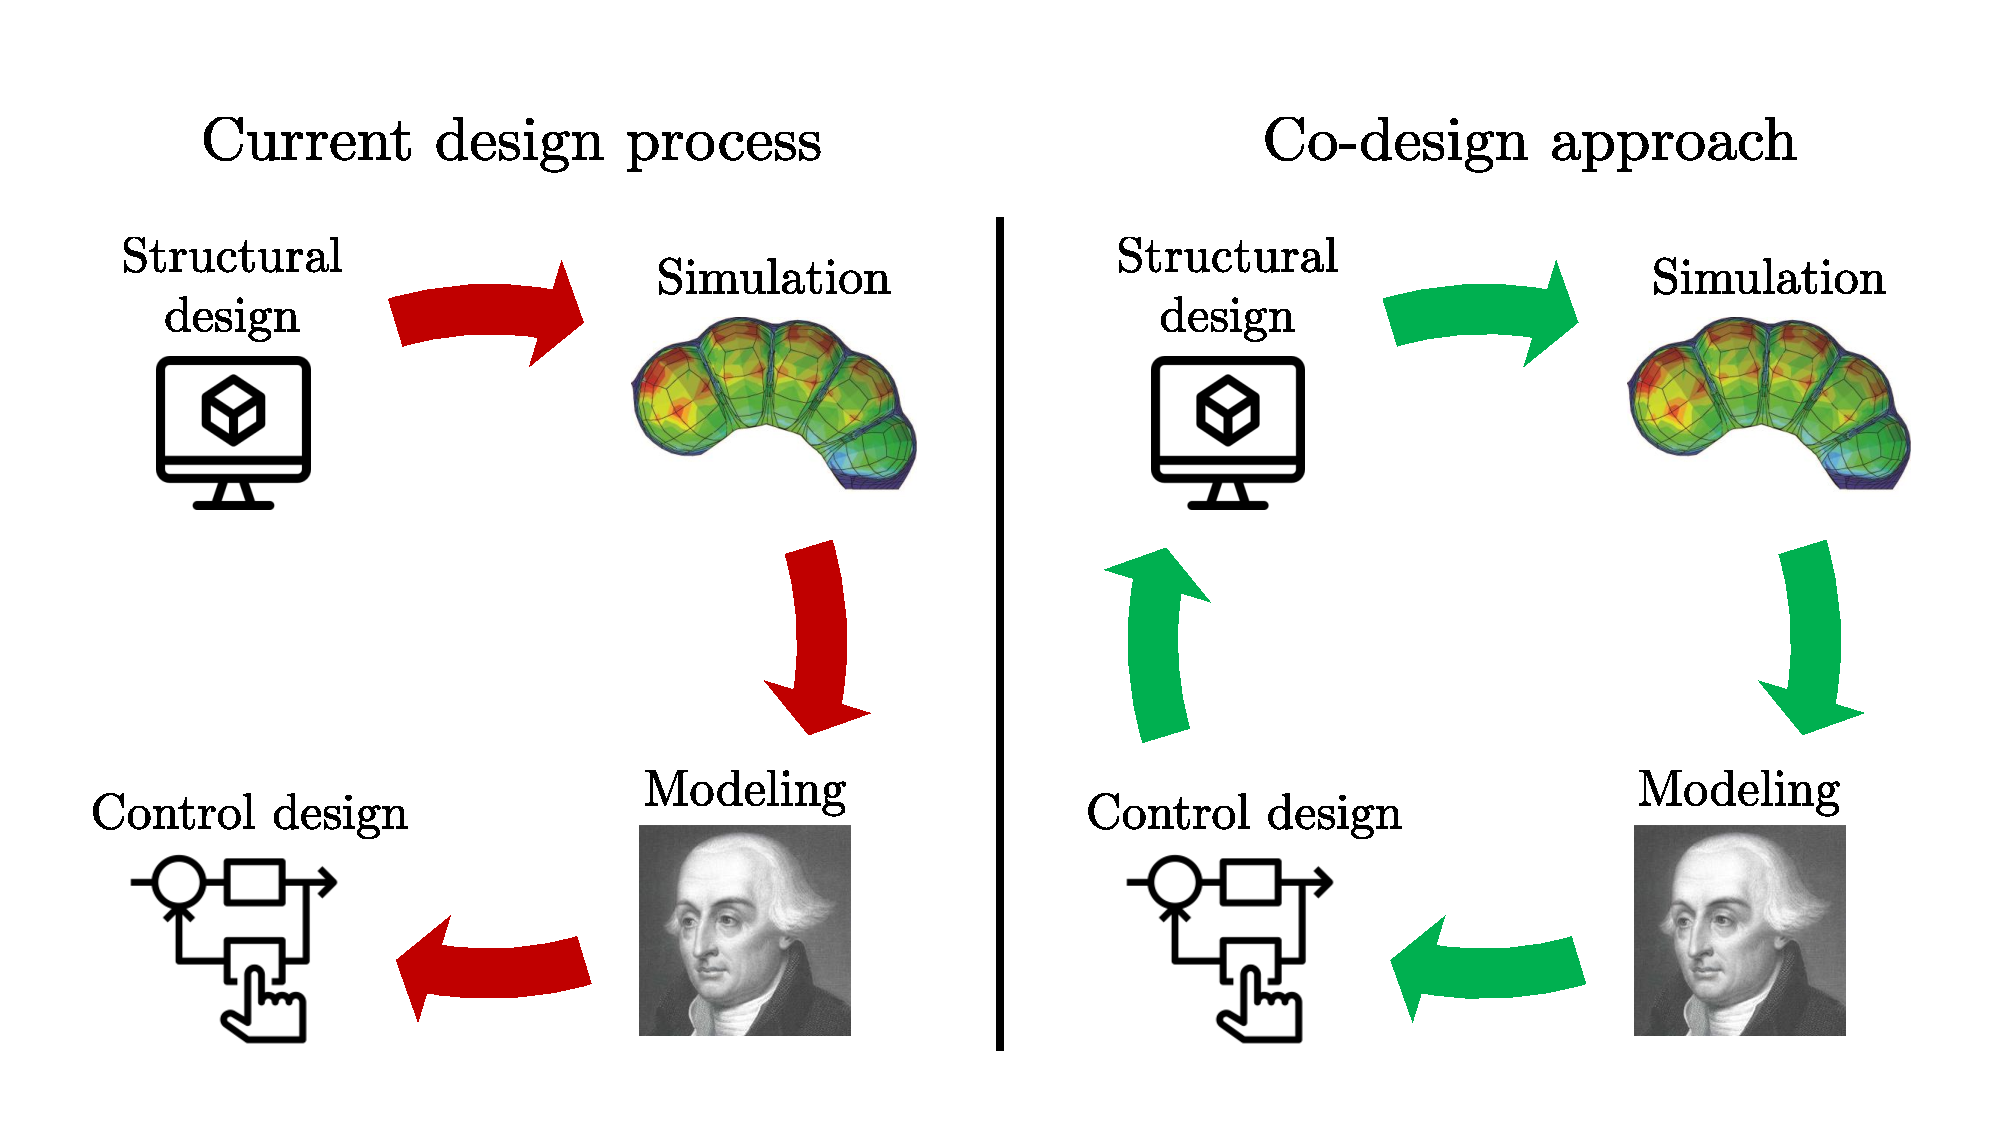
\includegraphics[width=0.6\linewidth]{conclusion/figures/future_work/co_design/motivation_co_design_v1_cropped.pdf}
    \caption{Traditional soft robot design follows a sequential process: first, the structure is created in \gls{CAD}; next, the robot’s behavior is simulated (for example, using \gls{FEM}); then, reduced-order kinematic and dynamic models are developed; and finally, the controller is designed based on these models. Moving forward, research should focus on a co-design approach that simultaneously optimizes the robot’s body (e.g., structure, actuation, sensors) and its brain (modeling, perception, control).}
    \label{fig:conclusion:future_work:co_design:motivation}
\end{figure}

% Instead, we strive in the future to co-design the body and the brain of the soft robot, leading to an optimal symbiosis of embodied~\citep{mengaldo2022concise} and computational intelligence, as visualized in Fig.~\ref{fig:conclusion:future_work:co_design:motivation}.
% While there has been some initial work on the co-design of soft robots~\citep{spielberg2019learning, bhatia2021evolution, van2022co, wang2022curriculum, wang2023preco, wang2024diffusebot}, the existing methods are too simplistic as they discretize the continuum into passive, actuated, and sensorized voxels or particles. 
% Therefore, the derived designs can only very rarely be realized in practice~\cite{legrand2023reconfigurable, wang2024diffusebot}.
% Additionally, most works train a learning-based (e.g., \gls{RL}) controller from scratch for each design iteration, creating a computational bottleneck for the co-design process~\cite{bhatia2021evolution, wang2022curriculum, wang2023preco}.
% We conclude that the immense computational demands of co-design currently limit its usefulness in practice as the design space that can actually be explored is small because of the limits of the available computing budget.
Looking ahead, our goal is to co-design the body and the brain of the soft robot, fostering an optimal integration of embodied~\citep{mengaldo2022concise} and computational intelligence, as illustrated in Fig.\ref{fig:conclusion:future_work:co_design:motivation}. Although some initial work on soft robot co-design exists~\citep{spielberg2019learning, bhatia2021evolution, van2022co, wang2022curriculum, wang2023preco, wang2024diffusebot}, these methods are often too simplistic, discretizing the continuum into passive, actuated, and sensorized voxels or particles. As a result, the derived designs are rarely practical~\citep{legrand2023reconfigurable, wang2024diffusebot}. Additionally, most studies train a learning-based controller (e.g., using \gls{RL}) from scratch for every design iteration, which creates a significant computational bottleneck in the co-design process~\citep{bhatia2021evolution, wang2022curriculum, wang2023preco}. We conclude that the high computational demands of co-design currently restrict its practical usefulness, limiting the scope of the design space that can be explored within available computing budgets.

% In the future, we should develop new, computationally tractable metrics that can assess, for example, the \emph{manufacturability}, \emph{observability}, \emph{controllability}, and \emph{safety) of the design, allowing the co-design process to communicate early signals to the optimizer which designs perform good or badly, instead of having to perform computationally demanding training of \gls{RL} controllers and slow \gls{FEM} simulations for each design to evaluate its fitness.
% Furthermore, rigid manipulators have fixed joints and links, allowing straightforward derivation of models essential for control. In contrast, the deformability of continuum soft robots complicates the accurate capturing of the system kinematics and dynamics with low-dimensional models~\citep{armanini2023soft}. Traditionally, experts have used trial and error to choose finite-dimensional backbone models (e.g., \gls{PCC}, \gls{PCS}, \gls{GVS}), but the best choice depends on the robot’s topology, actuation, and dynamics. Therefore, co-designing the reduced-order model with the hardware—and ideally automating this process—is crucial.
% Finally, the derivation of controllers with model-based approaches~\citep{della2023model}, instead of training a \gls{RL} policy for each design, could significantly speed up the co-design process.
% We discuss our perspective on the co-design of soft robots in more detail in Appendix~\ref{chp:apx:towardscodesign}.
Future research should develop and integrate computationally efficient metrics for manufacturability, observability, controllability, and safety to provide early feedback on the design to the optimizer—avoiding the need for costly \gls{RL} training and \gls{FEM} simulations for every design. While rigid manipulators benefit from fixed joints that simplify modeling, the deformability of soft robots complicates the creation of low-dimensional models~\citep{armanini2023soft}. Traditional trial-and-error methods for selecting backbone models (e.g., \gls{PCC}, \gls{PCS}, \gls{GVS}) depend heavily on a robot’s topology, actuation, and dynamics, making it essential to co-design reduced-order models with the morphology. Moreover, using model-based controllers rather than training a new \gls{RL} policy from scratch for each design could further accelerate the process. We discuss our perspective on soft robot co-design in more detail in Appendix~\ref{chp:apx:holisticcodesign}.

% \subsection{Integrating Stable Motion Primitives with Vision-Language-Action Models for Robust, Compliant, and Interpretable Motion Behavior}
\subsection{Towards Generalist Policies for Robust, Compliant, and Interpretable Motion Behavior by Integrating Stable Motion Primitives with Vision-Language-Action Models}
% In Chapter~\ref{chp:osmp}, we presented a motion policy based on \gls{SMP} for learning periodic motions from demonstration. Crucially, the parametrization of the motion policy with an interpretable dynamical system enables stability guarantees and compliant behavior.
% However, there currently exist several shortcomings that restrict the practicality of the approach: (a) most \gls{DMP}/\gls{SMP} approaches are currently limited to exhibiting one specific attractor class/type (e.g., fixed-point attractor, limit cycle, multistability), (b) crossing trajectories cannot be (readily) captured by a single \gls{DMP}, (c) they do not incorporate information about the environment into the decision making, and (d) they are only able to learn one or a few trajectories at a time.
% Instead, future work could combine \glspl{SMP} with modern \gls{VLM}/\gls{VLA} models: As visualized in Fig.~\ref{fig:conclusion:future_work:integrating_smps_with_vlas}, the \gls{VLM} would generate motion step sequences which subsequently would be tracked by a \gls{SMP} together with a low-level controller (e.g., an impedance controller).
% This can be seen, as demonstrated in Fig.\ref{fig:conclusion:future_work:integrating_smps_with_vlas:overview}, as a cascaded control scheme, with the low-level controller including configuration-space state feedback running at high frequencies (on the scale of \~\SI{1000}{Hz}), the \gls{SMP} providing references for the motion of the end-effector at a scale of \~\SI{100}{Hz}, and the \gls{VLM} running at \~\SI{10}{HZ} based on visual feedback of the situation and the environment, motion steps to the \gls{SMP}.
In Chapter~\ref{chp:osmp}, we introduced a motion policy based on \gls{SMP} for learning periodic motions from demonstrations. By parameterizing the policy with an interpretable dynamical system, we can ensure both stability and compliant behavior. However, several limitations currently restrict its practicality: (a) most \gls{DMP}/\gls{SMP} methods are confined to a single attractor type (e.g., fixed-point, limit cycle, multistability), (b) a single \gls{DMP} cannot readily capture intersecting trajectories, (c) information about the task setting and environment is not incorporated into decision-making, and (d) these methods typically learn only one or a few trajectories at a time.

To address these issues, future work might integrate \glspl{SMP} with modern \gls{VLM}/\gls{VLA} models. As shown in Fig.\ref{fig:conclusion:future_work:integrating_smps_with_vlas}, a \gls{VLM} could generate sequences of motion steps that are then tracked by an \gls{SMP} combined with a low-level controller (e.g., an impedance controller). This setup forms a cascaded control scheme, illustrated in Fig.\ref{fig:conclusion:future_work:integrating_smps_with_vlas:overview}: a low-level controller with configuration-space state feedback runs at high frequencies (around \SI{1000}{Hz}), the \gls{SMP} supplies end-effector motion references at approximately \SI{100}{Hz}, and the \gls{VLM} operates at about \SI{10}{Hz}, processing visual feedback to issue motion steps to the \gls{SMP}.

\begin{figure}[ht]
    \centering
    \subfigure[Overview: Integration of Stable Motion Primitives (SMPs) with Vision-Language-Action (VLAs) Models]{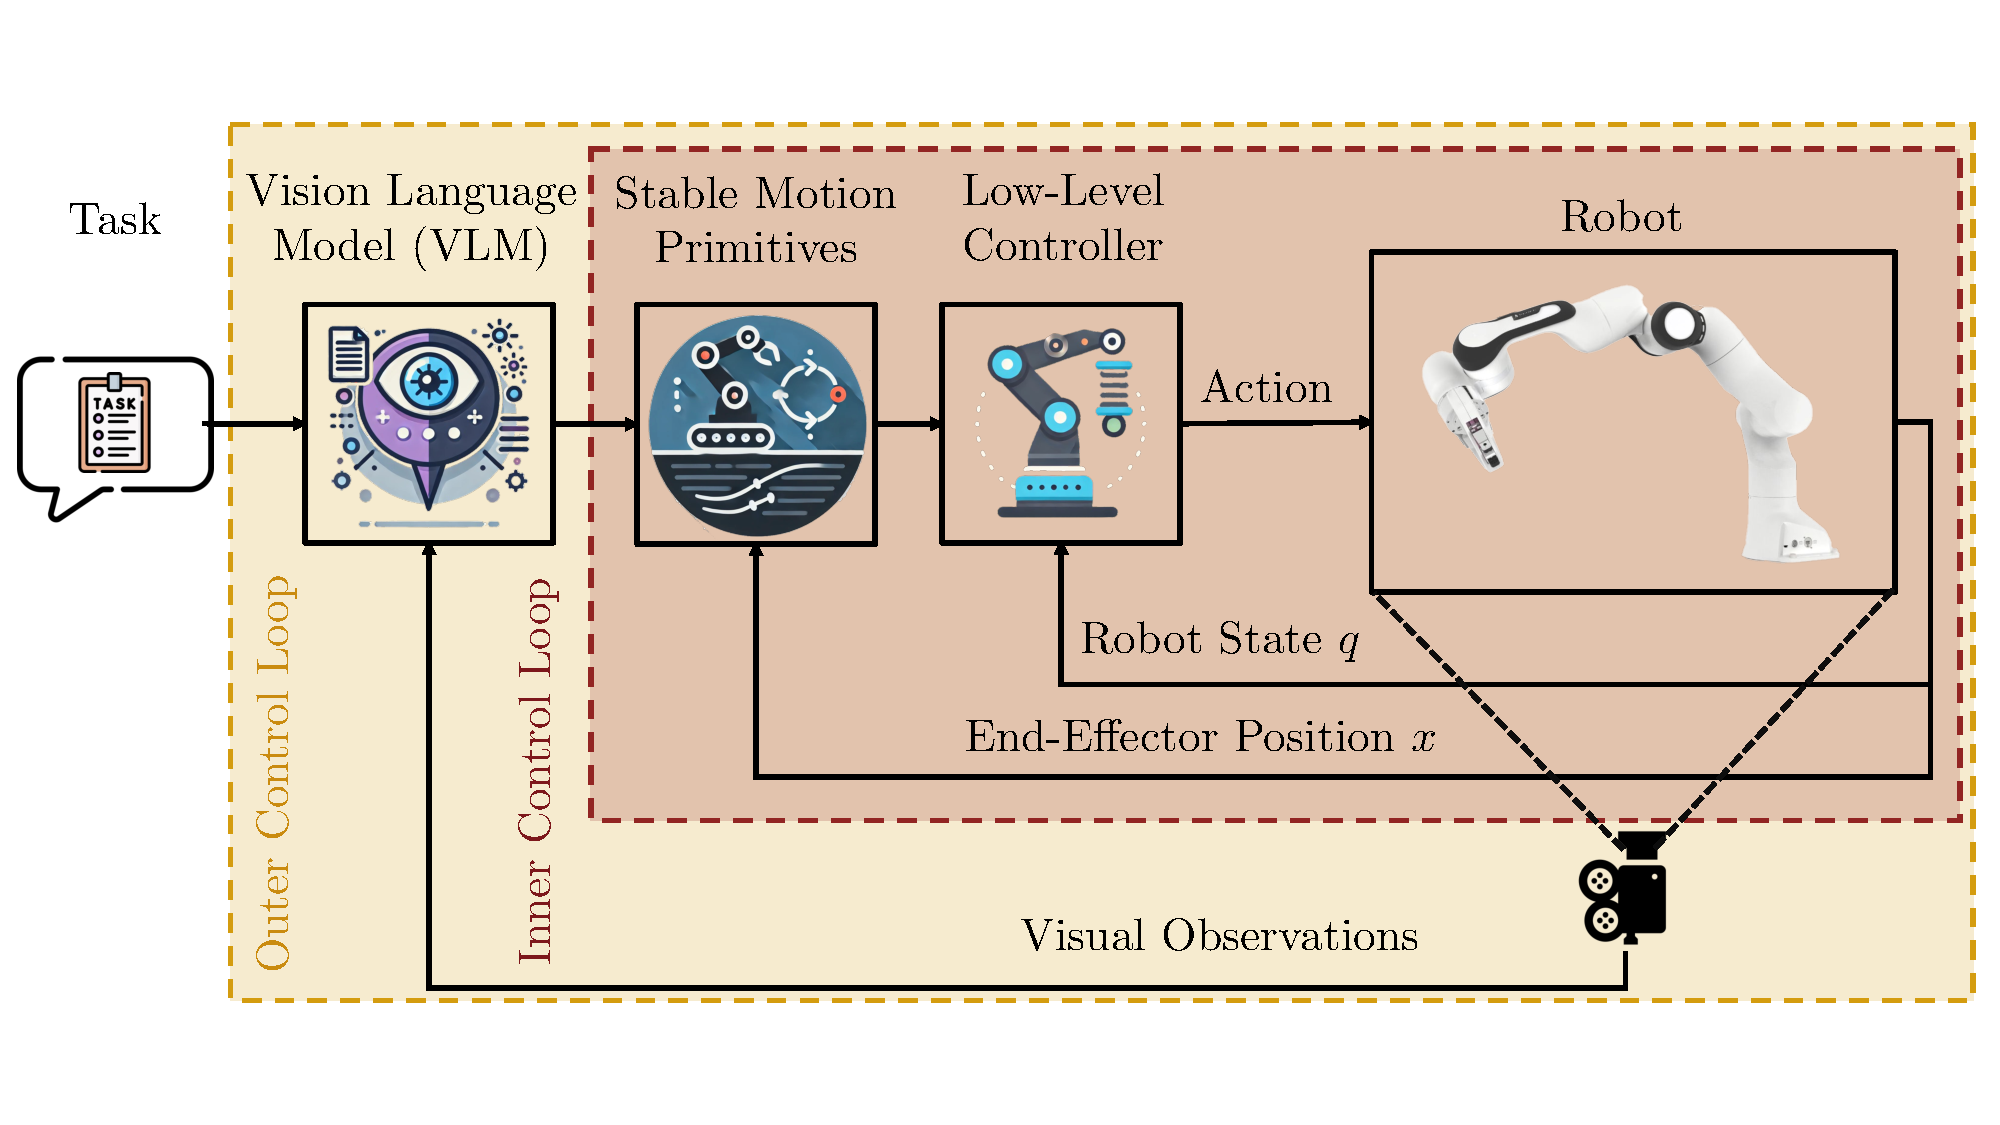
\includegraphics[width=0.65\linewidth]{conclusion/figures/future_work/integrating_smps_with_vlms/smps_and_vlms_v1_cropped.pdf}\label{fig:conclusion:future_work:integrating_smps_with_vlas:overview}}\\
    \subfigure[Hierarchical Planning with \glspl{VLM}]{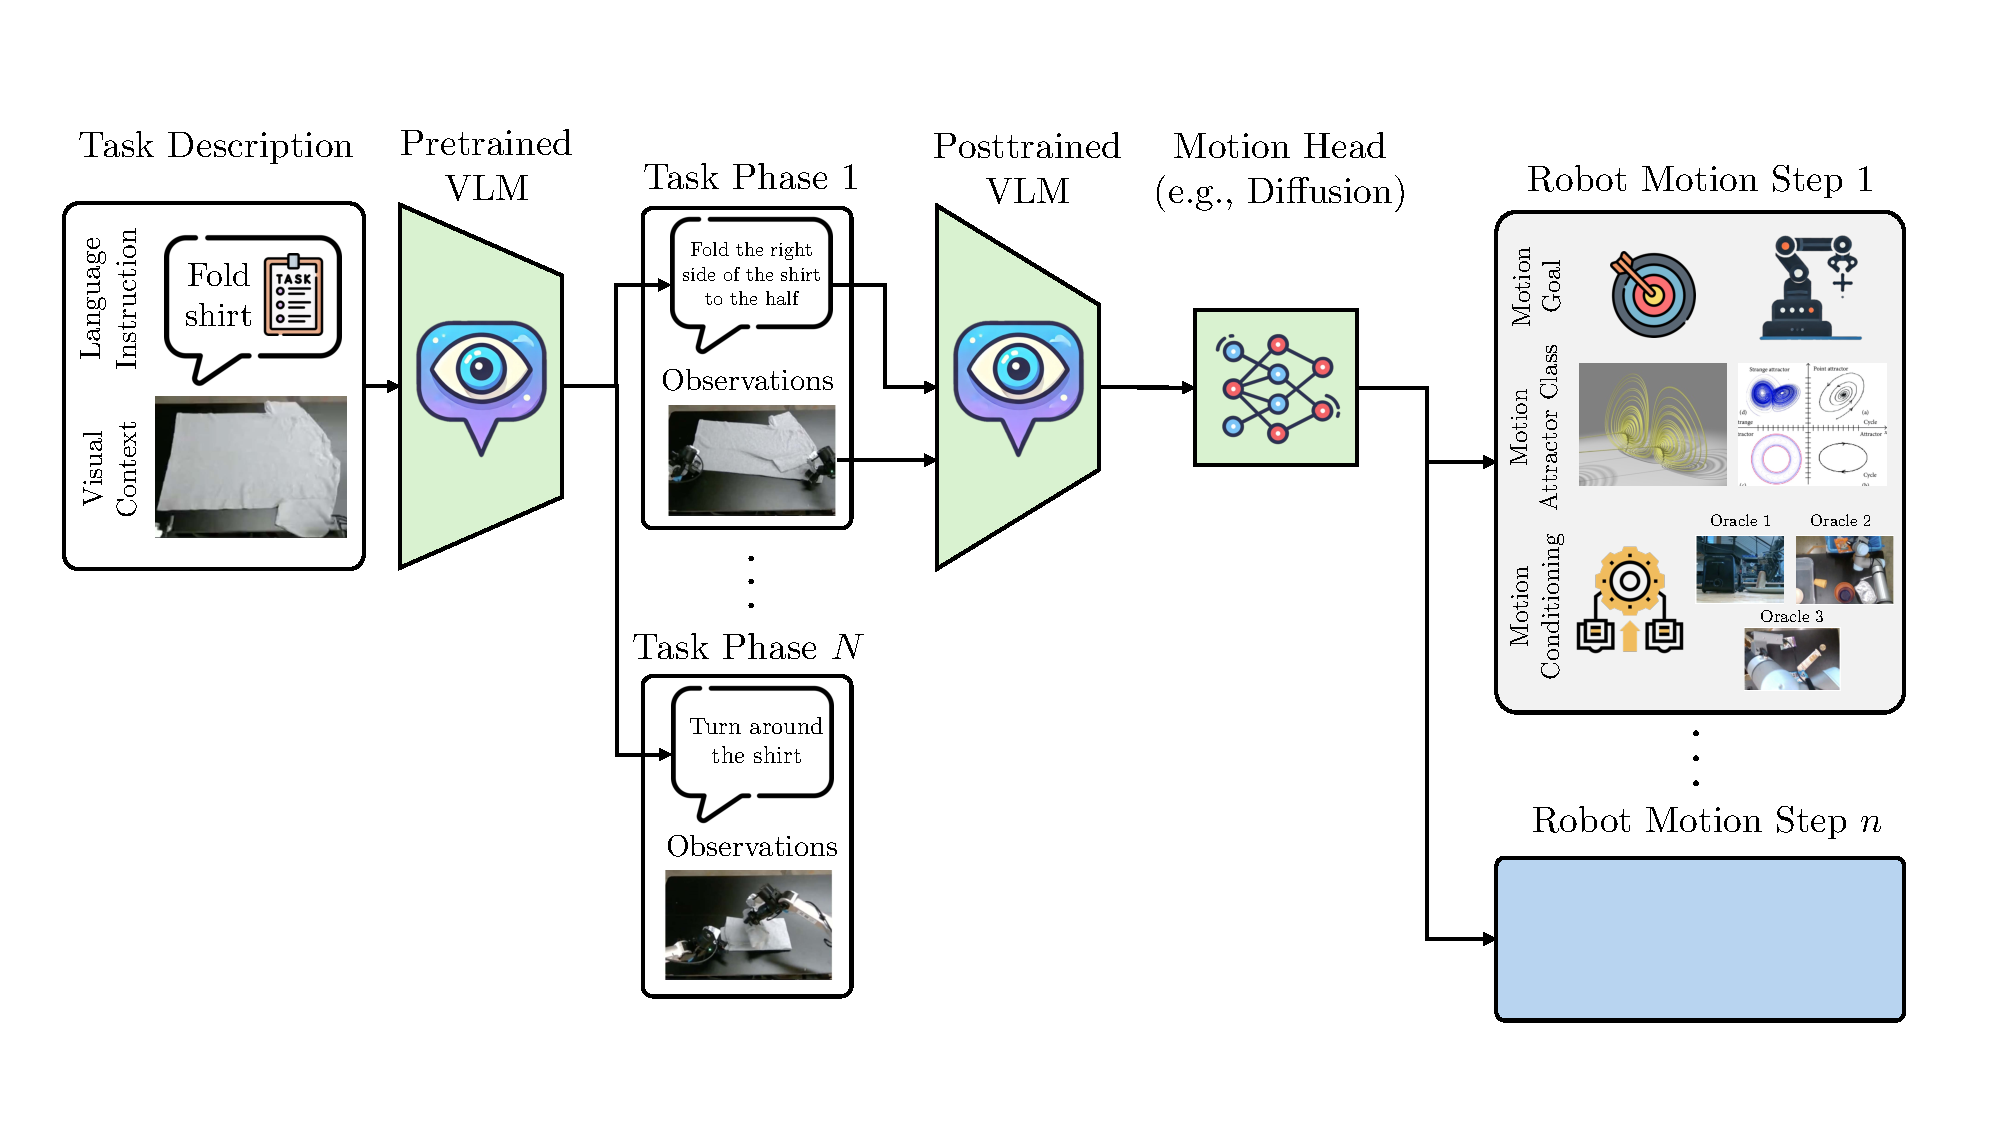
\includegraphics[width=0.85\linewidth]{conclusion/figures/future_work/integrating_smps_with_vlms/hierarchical_planning_with_vlms_v1_cropped.pdf}\label{fig:conclusion:future_work:integrating_smps_with_vlas:hierarchical_planning}}
    \subfigure[Expressive \glspl{SMP}]{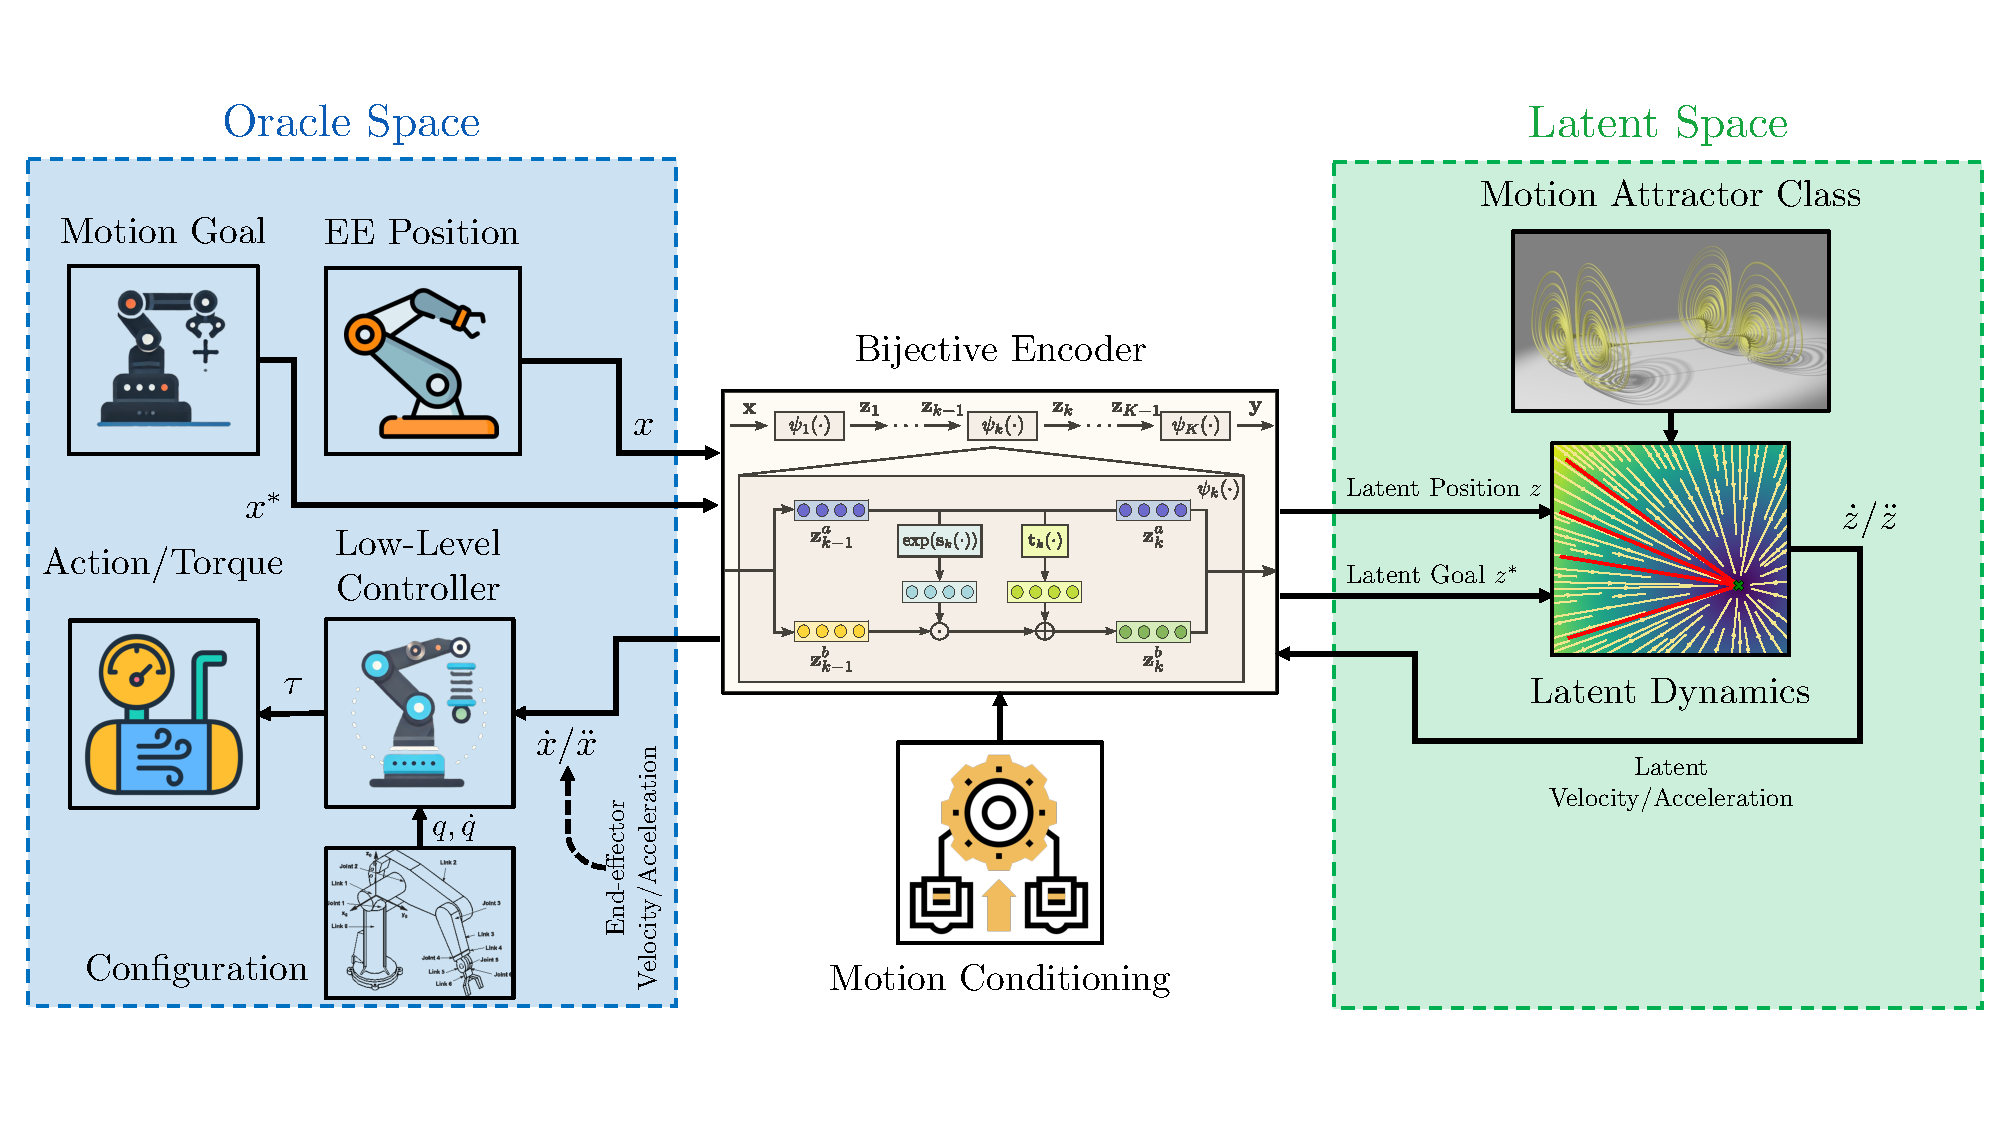
\includegraphics[width=0.80\linewidth]{conclusion/figures/future_work/integrating_smps_with_vlms/expressive_smps_v1_cropped.pdf}\label{fig:conclusion:future_work:integrating_smps_with_vlas:expressive_smps}}
    \caption{Concept for the Integrating \glspl{SMP} with \glspl{VLA} models: The \gls{VLM}, composed of a pretrained and posttrained part, receives, possibly multimodal, task instructions, and its motion head translates them into robot motion steps instead of directly outputting actions. These robot motion steps, consisting of, for example, a motion goal, the motion attractor class, and conditioning on the demonstration/oracle, then shape the behavior of the motion policy parametrized by a dynamical system (i.e., a \gls{SMP}).}
    \label{fig:conclusion:future_work:integrating_smps_with_vlas}
\end{figure}

% Specifically, we envision, as shown in Fig.~\ref{fig:conclusion:future_work:integrating_smps_with_vlas:hierarchical_planning}, employing a hierarchical approach~\citep{haresh2024clevrskills} for dividing a high-level task, such as folding laundry, in task phases (e.g., folding the right side of the shirt to the half) and motion steps, using both pretrained and posttrained \glspl{VLM}.
% \footnote{Here, \emph{pretrained} refers to a \gls{VLM} that was pretrained on internet-scale data and large-scale cross-embodiment datasets~\citep{o2024open, kim2024openvla}. On the other hand, \emph{postrained} refers to fine-tuning such a \emph{pretrained} model on small-scale, high-quality datasets that directly the robot embodiment and task on which the model should operate on~\citep{black2024pi0}.}
% The connection between the \glspl{VLM} and the \gls{SMP} is made through a motion head network, for example, based on diffusion policies~\citep{chi2023diffusion}, that predicts the necessary robot step of the robot consisting of a motion goal/waypoints, the \gls{SMP} attractor class (e.g., fixed point, limit cycle, multistability), and conditioning of the \gls{SMP} encoder on a motion demonstration seen during training.
% Fig.~\ref{fig:conclusion:future_work:integrating_smps_with_vlas:expressive_smps} visualizes how this conditioning mechanism allows to make \glspl{SMP} more expressive and to capture many motions in one policy.
% During inference, both the motion goal $x^*$ and the current end-effector position $x$ are passed through the bijective encoder~\citep{rana2020euclideanizing}, and, with that, encoded in latent space positions $z^*$ and $z$, respectively. 
% The latent dynamics, governed by the latent goal and the chosen motion attractor class, then provide us with a latent velocity $\dot{z}$, which is subsequently projected back into oracle space using the inverse Jacobian of the encoder.
% This velocity reference can then be tracked by a low-level controller that computes the actuation commands.
More specifically, as depicted in Fig.\ref{fig:conclusion:future_work:integrating_smps_with_vlas:hierarchical_planning}, we envision a hierarchical approach~\citep{haresh2024clevrskills} that breaks down a high-level task—such as folding laundry—into task phases (e.g., folding the right side of a shirt halfway) and individual motion steps, utilizing both pretrained and posttrained \glspl{VLM}\footnote{Here, \emph{pretrained} refers to a \gls{VLM} trained on internet-scale data and large cross-embodiment datasets~\citep{o2024open, kim2024openvla}, while \emph{posttrained} indicates a version fine-tuned on smaller, high-quality datasets specific to the robot embodiment and task~\citep{black2024pi0}.}. The connection between the \glspl{VLM} and the \gls{SMP} is facilitated by a motion head network—potentially based on diffusion policies~\citep{chi2023diffusion}—that predicts the necessary robot step, including a motion goal or waypoints, the corresponding \gls{SMP} attractor type (e.g., fixed-point, limit cycle, multistability), and the conditioning of the \gls{SMP} encoder on a motion demonstration from training. Figure~\ref{fig:conclusion:future_work:integrating_smps_with_vlas:expressive_smps} illustrates how this conditioning mechanism enhances the expressiveness of \glspl{SMP}, enabling a single policy to represent a wide range of motions. During inference, both the motion goal $x^\mathrm{d}$ and the current end-effector position $x$ are passed through a bijective encoder~\citep{rana2020euclideanizing}, which maps them into latent space coordinates $z^\mathrm{d}$ and $z$, respectively. The latent dynamics—governed by the latent goal and the selected attractor type—yield a latent velocity $\dot{z}$, which is then projected back into the original space using the encoder’s inverse Jacobian. A low-level controller subsequently tracks this velocity reference by computing the required actuation commands.

% This strategy could allow us to increase the expressiveness and generalization performance of \glspl{SMP}-based policies by combining them with \gls{SOTA} while preserving some of the insight and stability guarantees that \glspl{SMP} exhibit. 
% Notably, these characteristics would separate it from modern \glspl{VLA} policies~\citep{black2024pi0}, which do not allow for any insight into the action generation nor exhibit any stability guarantees.
This strategy has the potential to enhance the expressiveness and generalization of \gls{SMP}-based policies by combining them with state-of-the-art models while still preserving the interpretability and stability guarantees inherent to \glspl{SMP}. These features notably distinguish our approach from current \gls{VLA} policies~\citep{black2024pi0, kim2024openvla}, which generally do not provide insight into the action generation process or offer stability guarantees.